\section{Feature Engineering}
Our team members extracted 7 feature sets, namely F1, F2, F3, F4, F5, F6, and F7 from raw data independently.

\subsection{Data Sets}
Activity logs of 200,906 enrollments from 112,448 students across 39 courses are provided.
Each activity is described by 6 fields of the username, course ID, timestamp, source, event, and object. 
For each object, 3 additional fields of the category, children, and start date are provided.
The training set consists of 8,157,278 logs from 120,543 enrollments with the target variable indicating if a student dropped out.  
The test set consists of 5,387,848 logs from 80,363 enrollments.
The full description of the data sets is available in \cite{kddcup2015_data}. In general, this data can be organized in three dimension space, object, time, and event as shown in Figure~\ref{fig:cube}. Feature engineering tasks were carried out based on these views.

\begin{figure}[!t]
	\caption{Data Cube}
	\centering
	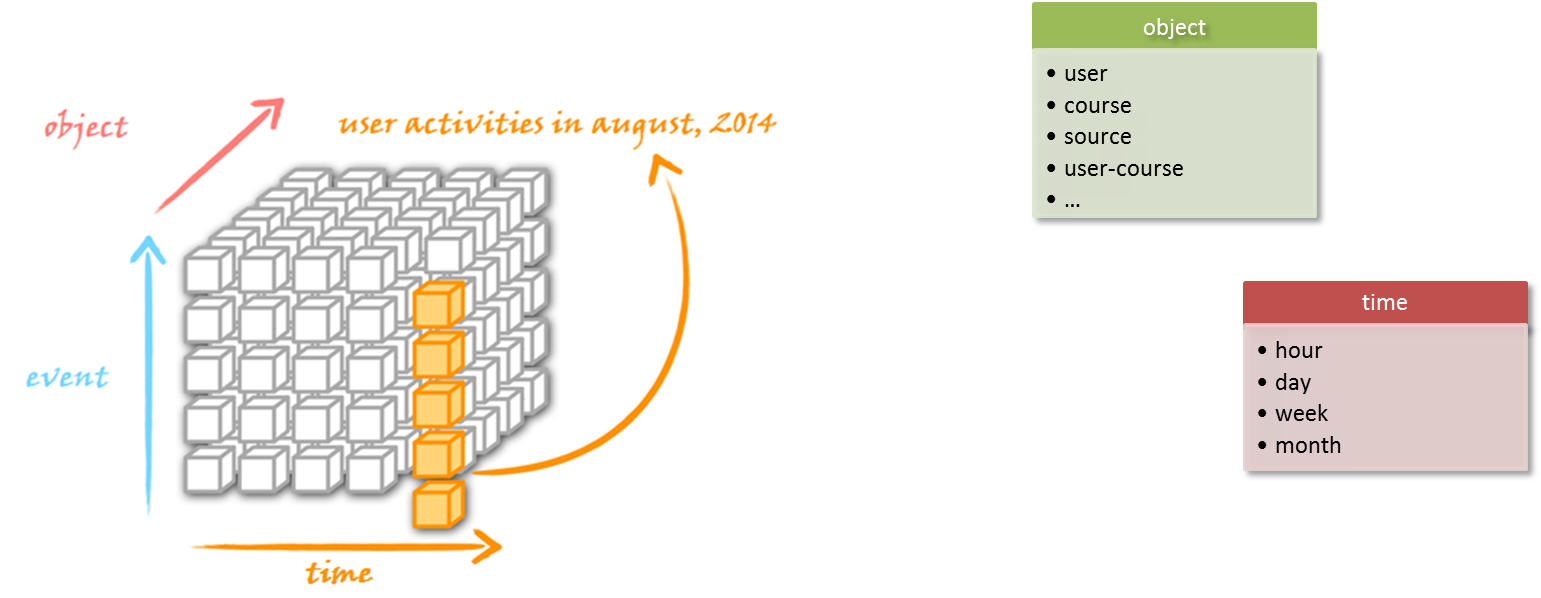
\includegraphics[width=0.5 \textwidth]{cube}
	\label{fig:cube}
\end{figure}


\subsection{Common Features}
Attributes available from raw data
There are common features across 7 feature sets, F1 through F7 as follows:
\begin{itemize}
	\item Number of objects
	\item Number of events
	\item Aggregation features of features above
\end{itemize}
The common features can be generated using cube operations. Figure~\ref{fig:slice} shows an example how weekly and monthly count features are calculated. First, the data is cut using object dimension. In this case, we choose to generate feature for users. Next, we select an event "navigate" in the event space to generate a time series presenting "navigate" event over the time. Finally, the drill-down operation is used to generate monthly or weekly count features.

\begin{figure}[!t]
	\caption{Slice and Dice}
	\centering
	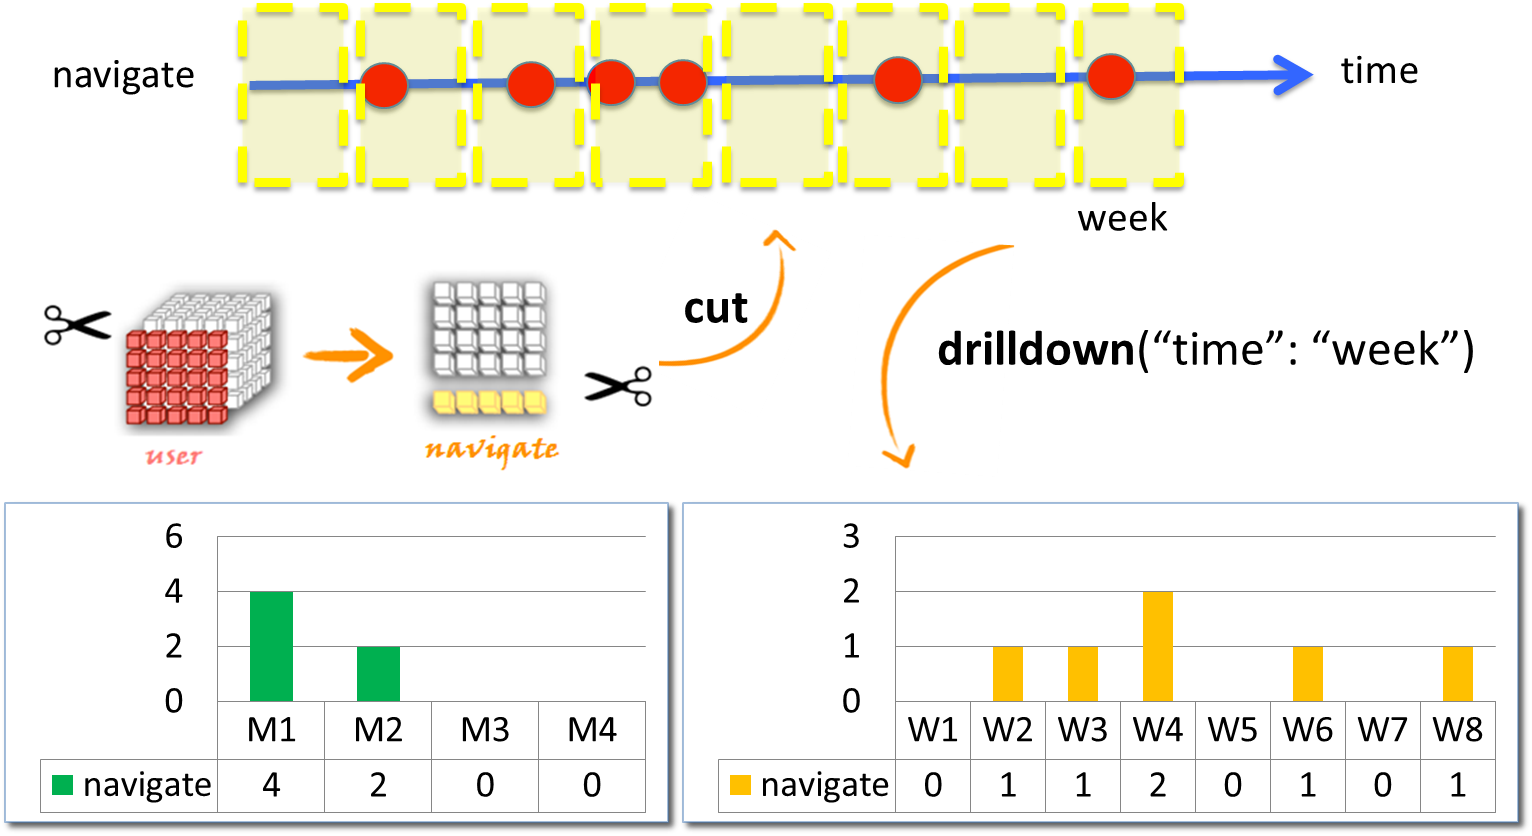
\includegraphics[width=0.5 \textwidth]{slice_and_dice}
	\label{fig:slice}
\end{figure}

\subsection{F1}

The feature set F1 is generated by Chen and Ozaki and includes features as follows:

\begin{itemize}
  \setlength\itemsep{0em}
  \item Enrollment-based features (No.1-8)
  \item Username-based features (No.9-18)
  \item Username-based features for each courses (No.19-25) 
  \item Features based on 10 days after the end date of course (No.26-35)
  \item Features based on 1 day after the end date of a course (No.36-45)
  \item Day-level features (No.46)
  \item Day-level features using target variables (No.47-58)
\end{itemize}

Table~\ref{tb:skfeature} shows the full list of features in F1.

\subsection{F2}
The feature set F2 is generated by Yan and Zhou and includes features as follows:
\begin{itemize}
  \setlength\itemsep{0em}
  \item Visit time(hour, day) set features (including time span and max absent days)
  \item Act(event, object) counting features (some uses missed content counts)
  \item Course drop rate
  \item Number of courses the user enrolled
  \item Minimum time interval between time points(first visit, last visit, course begin, course end, 10 days after course end) of current course and another enrolled course
  \item Active days between course end and 10 days after course end
  \item Active days between last visit and course end
  \item Number of courses ended after current course end
\end{itemize}

Table~\ref{tb:rwfeature} shows the full list of features in F2.

\subsection{F3}
The feature set F3 is generated by Nguyen, and are categorized into 3 groups of the count, aggregation, and date features.

\subsubsection{Count Features}
There are a few entities such as user, course, and object in the training dataset.  Combining these entities together, we have user activities or events.  The simplest way to generate features from these events is to count the number of times an entity engaging in the event. The motivation is that the more a user participate in course, the less likely she drop out the course. Table~\ref{tb:tnfeature1} shows the list of count features in F1. 

\begin{center}
	\begin{table}[ht]
		\begin{minipage}{0.5 \textwidth}
			{
				\small
				\hfill{}
				\begin{tabular}{|l|l|l|}
					\hline
					\textbf{No.}	&\textbf{Description}\tabularnewline \hline
					1 			& The log count of each user \tabularnewline
					2 			& The log count of each course \tabularnewline
					3			& The log count of each event \tabularnewline
					4 			& The log count of each user per week \tabularnewline
					5 			& The log count of each user per two weeks \tabularnewline
					6 			& The log count of each user per weekday \tabularnewline
					7 			& The log count of each user per month\tabularnewline
					8 			& The log count of each course per week \tabularnewline
					9 			& The log count of each course per two weeks \tabularnewline
					10 			& The log count of each course per weekday\tabularnewline
					11 			& The log count of each course per month \tabularnewline
					12 			& The log count of each event per week \tabularnewline
					13 			& The log count of each event per two weeks \tabularnewline
					14 			& The log count of each event per weekday \tabularnewline
					15 			& The log count of each event per month \tabularnewline
					\hline
				\end{tabular}
			}
			\hfill{}
			\caption{List of count features in F3.}
			\label{tb:tnfeature1}
		\end{minipage}
	\end{table}
\end{center}

\subsubsection{Aggregation Features}
Aggregation features are calculated based on count features. Usually, each course would have a fixed schedule for users to study. Therefore, students enrolled in the course must have consistent activity patterns.  Aggregation features would measure the stability of course engagement.  These features are minimum, mean, median, maximum, and standard deviation of count features on date basis such as weekly, monthly, etc.

\subsubsection{Date Features}
To capture how often users participate in a certain course, we generated date features. Date features can be time span among user activities as well as time span from last activity and last course date. Table~\ref{tb:tnfeature3} shows the list of date features in F3. 

\begin{center}
	\begin{table}[ht]
		\begin{minipage}{0.5 \textwidth}
			{
				\small
				\hfill{}
				\begin{tabular}{|l|l|l|}
					\hline
					\textbf{No.}	&\textbf{Description}\tabularnewline \hline
					1 			& Min time span among activities \tabularnewline
					2 			& Max time span among activities \tabularnewline
					3 			& Mean time span among activities \tabularnewline
					4 			& Time span from the last activity and last course date \tabularnewline
					5 			& The number of unique activity days of each user \tabularnewline
					\hline
				\end{tabular}
			}
			\hfill{}
			\caption{List of date features in F3.}
			\label{tb:tnfeature3}
		\end{minipage}
	\end{table}
\end{center}

\subsection{F4}
The feature set F4 is generated by Jahrer, and includes features as follows:

\begin{itemize}
  \setlength\itemsep{0em}
  \item uID (0-112,447)
  \item cID (112,448-112,486)
  \item uIDcnt (112,487-112,487)
  \item eIDcnt (112,488-112,488)
  \item eID $\rightarrow$ sID (112,489-112,490)
  \item eID $\rightarrow$ evID (11,2491-112,497)
  \item eID $\rightarrow$ oIDCnt (112,498-139,443)
  \item eID $\rightarrow$ tIDCnt (139,444-139,635)
  \item uID: floor(log(dateSpan$^2$+1)) (139,636-140,635)
  \item uID $\rightarrow$ log(time diff to obj start+1) (140,636-140,636)
  \item eID $\rightarrow$ dateVec diff stats (140,637-140,649)
\end{itemize}

\subsection{F5}
The feature set F5 is generated by Bay, and includes features as follows:
\begin{itemize}
  \setlength\itemsep{0em}
  \item Course ID - One-hot-encoded course\_id
  \item Source time counts  by enrollment - The log count of each source type per day for each enrollment
  \item Source time counts by course id - The log count of each source type per day for each course id
  \item Event time counts by enrollment - The log count of each event type per day for each enrollment
  \item Event time counts by course id - The log count of each event type per day for each course id

\end{itemize}

\subsection{F6}
The feature set F6 is generated by Lee, and includes features as follows:

\begin{itemize}
  \setlength\itemsep{0em}
  \item User ID (20,113) - One-hot-encoded username. Usernames appearing less than 100 times in training log data are grouped together as one user ID. 
  \item Course ID (39) - One-hot-encoded course\_id.
  \item Source Event (10) - One-hot-encoded combination of source and event.
  \item Object ID (3,554) - One-hot-encoded object.  Objects appearing less than 100 times in training log data are grouped together as one object ID.
  \item Count (1) - Number of log entries for an hour\_id.
  \item Object Category (6) - Number of log entries with an object category for an enrollment\_id.
  \item Number of Children Objects (7) - One-hot-encoded total number of object's children for an enrollment\_id.
  \item Object Timespan (10) - One-hot-encoded timespan in days between object's start date and last day of the class
  \item Day of Class (30) - One-hot-encoded day of the class
  \item Week of Class (4) - One-hot-encoded week of the class
  \item End Month of Class (7) - One-hot-encoded end month of the class
  \item Object Started in Dropout Period (2) - Binary variable that is 1 if object started after but before 10 days after last day of the class and 0 otherwise.
\end{itemize}

\subsection{F7}

The feature set F7 is generated by Ozaki, and encodes target variables for each days.

\begin{itemize}
  \setlength\itemsep{0em}
  \item For each 10 days after the end date of the course, number of active enrollment\_id, which target variables are 1 in the training set, enrolled by an username.
  \item For each 10 days after the end date of the course, number of active enrollment\_id, which target variables are 0 in the training set, enrolled by an username.
  \item For each 10 days after the end date of the course, number of active enrollment\_id (in this case, days between last access and the end date of the course are also counted for active days), which target variables are 1 in the training set, enrolled by an username.
  \item For each 10 days after the end date of the course, number of active enrollment\_id (in this case, days between last access and the end date of the course are also counted for active days), which target variables are 0 in the training set, enrolled by an username.
  \item For each 14 days before the end date of the coruses, number of active enrollment\_id, which target variables are 1 in the training set, enrolled by an username.
  \item For each 14 days before the end date of the coruses, number of active enrollment\_id, which target variables are 0 in the training set, enrolled by an username.
  \item For each 14 days before the end date of the coruses, number of active enrollment\_id (in this case, days between last access and the end date of the course are also counted for active days), which target variables are 1 in the training set, enrolled by an username.
  \item For each 14 days before the end date of the coruses, number of active enrollment\_id (in this case, days between last access and the end date of the course are also counted for active days), which target variables are 0 in the training set, enrolled by an username.
\end{itemize}
